%%%%%%%%%%%%%%%%%%%%%%%%%%%%%%%%%%%%%%%%%
% Beamer Presentation
% LaTeX Template
% Version 1.0 (10/11/12)
%
% This template has been downloaded from:
% http://www.LaTeXTemplates.com
%
% License:
% CC BY-NC-SA 3.0 (http://creativecommons.org/licenses/by-nc-sa/3.0/)
%
%%%%%%%%%%%%%%%%%%%%%%%%%%%%%%%%%%%%%%%%%

%----------------------------------------------------------------------------------------
%	PACKAGES AND THEMES
%----------------------------------------------------------------------------------------

\documentclass{beamer}

\mode<presentation> {

% The Beamer class comes with a number of default slide themes
% which change the colors and layouts of slides. Below this is a list
% of all the themes, uncomment each in turn to see what they look like.

%\usetheme{default}
%\usetheme{AnnArbor}
%\usetheme{Antibes}
%\usetheme{Bergen}
%\usetheme{Berkeley}
%\usetheme{Berlin}
%\usetheme{Boadilla}
%\usetheme{CambridgeUS}
%\usetheme{Copenhagen}
%\usetheme{Darmstadt}
%\usetheme{Dresden}
%\usetheme{Frankfurt}
%\usetheme{Goettingen}
%\usetheme{Hannover}
%\usetheme{Ilmenau}
%\usetheme{JuanLesPins}
%\usetheme{Luebeck}
\usetheme{Madrid}
%\usetheme{Malmoe}
%\usetheme{Marburg}
%\usetheme{Montpellier}
%\usetheme{PaloAlto}
%\usetheme{Pittsburgh}
%\usetheme{Rochester}
%\usetheme{Singapore}
%\usetheme{Szeged}
%\usetheme{Warsaw}

% As well as themes, the Beamer class has a number of color themes
% for any slide theme. Uncomment each of these in turn to see how it
% changes the colors of your current slide theme.

%\usecolortheme{albatross}
%\usecolortheme{beaver}
%\usecolortheme{beetle}
%\usecolortheme{crane}
%\usecolortheme{dolphin}
%\usecolortheme{dove}
%\usecolortheme{fly}
%\usecolortheme{lily}
%\usecolortheme{orchid}
%\usecolortheme{rose}
%\usecolortheme{seagull}
%\usecolortheme{seahorse}
%\usecolortheme{whale}
%\usecolortheme{wolverine}

%\setbeamertemplate{footline} % To remove the footer line in all slides uncomment this line
%\setbeamertemplate{footline}[page number] % To replace the footer line in all slides with a simple slide count uncomment this line

%\setbeamertemplate{navigation symbols}{} % To remove the navigation symbols from the bottom of all slides uncomment this line
}

\usepackage{graphicx} % Allows including images
\usepackage{booktabs} % Allows the use of \toprule, \midrule and \bottomrule in tables
\usepackage{multirow}
\usepackage{adjustbox}
\usepackage{array}
\usepackage{tikz}
\usepackage{soul}
\usetikzlibrary{shapes.geometric, arrows, positioning, fit}
\usepackage[latin1]{inputenc}
\newcommand{\xmark}{\textcolor{red}{\text{\sffamily X}}}
\newcommand{\cmark}{\textcolor{green}{\checkmark}}
\newcommand{\tr}{\text{tr}}
\newcommand{\E}{\textbf{E}}
\newcommand{\diag}{\text{diag}}
\newcommand{\argmax}{\text{argmax}}
\newcommand{\argmin}{\text{argmin}}
\newcommand{\Cov}{\text{Cov}}
\newcommand{\Var}{\text{Var}}
\newcommand{\Vol}{\text{Vol}}
\newcommand{\bx}{\boldsymbol{x}}
\newcommand{\by}{\boldsymbol{y}}
\newcommand{\bX}{\boldsymbol{X}}
\newcommand{\bY}{\boldsymbol{Y}}
\sethlcolor{gray}
\makeatletter
\newcommand\SoulColor{%
  \let\set@color\beamerorig@set@color
  \let\reset@color\beamerorig@reset@color}
\makeatother
\definecolor{color1}{RGB}{128,13,13}
\definecolor{color2}{RGB}{70,128,13}
\definecolor{color3}{RGB}{13,128,128}
\definecolor{color4}{RGB}{70,13,128}

%tikz stufff


%----------------------------------------------------------------------------------------
%	TITLE PAGE
%----------------------------------------------------------------------------------------


%Extrapolating prediction error for 'extreme' multi-class classification

%with Rakesh Achanta and Yuval Benjamini

%'Extreme' classification refers to the classification with extremely
%large (on the order of millions) of labels, such as in photo or
%website annotation.  A natural question in these settings is whether
%the data is sufficiently rich to support high-accuracy classification
%with such a large label space.  Therefore, in this work, we address
%the question of predicting how well a classifier will scale with an
%increased number of classes, based on its performance in a smaller but
%representative classification problem. Under the assumption that the
%classes are sampled exchangeably, and under the assumption that the
%classifier is based on marginal probabilities (e.g. QDA or Naive
%Bayes), we derive a method for performance extrapolation based on
%unbiased estimation. We investigate the robustness of our methods to
%non-marginal classifiers in simulations and one optical character
%recognition example.


% Image sources
% http://sociable.co/social-media/how-to-disable-facebook-facial-recognition/
% https://alexanderskv.wordpress.com/2012/06/04/facial-recognition/
% https://medium.com/@ageitgey/machine-learning-is-fun-part-4-modern-face-recognition-with-deep-learning-c3cffc121d78#.fzgvan3ii

\title[Multi-class error]{Extrapolating prediction error for `extreme' multi-class classification}

\author{Charles Zheng} % Your name
\institute[Stanford] % Your institution as it will appear on the bottom of every slide, may be shorthand to save space
{Stanford University}
\date{\today} % Date, can be changed to a custom date

\begin{document}

\begin{frame}
\titlepage % Print the title page as the first slide
(Joint work with Rakesh Achanta and Yuval Benjamini.)
\end{frame}


\begin{frame}
\frametitle{Multi-class classification}
\begin{columns}
\begin{column}{0.5\textwidth}
\begin{center}
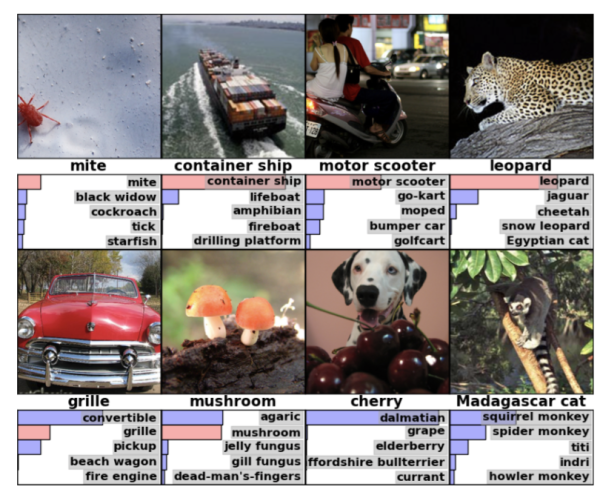
\includegraphics[scale = 0.4]{imagenet-fig4l.png}
\end{center}
\vspace{0.2in}
\tiny{from Krizhevsky et al. 2012}
\end{column}
\begin{column}{0.5\textwidth}
\begin{itemize}
\item MNIST digit recognition: 10 categories
\item Human motion database: 51 categories
\item ImageNet: 22,000 categories
\item Wikipedia: 325,000 categories
\end{itemize}
\end{column}
\end{columns}
\end{frame}

\begin{frame}
\frametitle{Facial recognition}
\begin{itemize}
\item Used to tag images in software, security \pause
\item Preprocessing
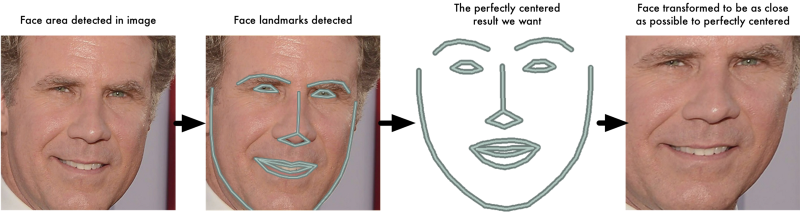
\includegraphics[scale = 0.4]{face_alignment.png}
\pause
\item Feature extraction
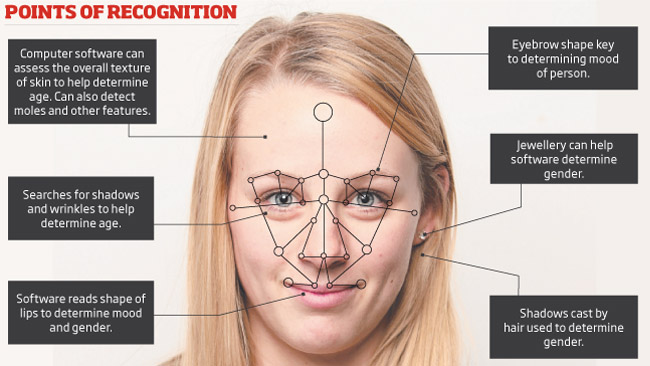
\includegraphics[scale = 0.4]{facerec_features.jpg}
\end{itemize}
\end{frame}


\begin{frame}
\frametitle{Accuracy vs. number of classes}
%Kay (2008) image identification task in functional MRI.
\begin{center}
%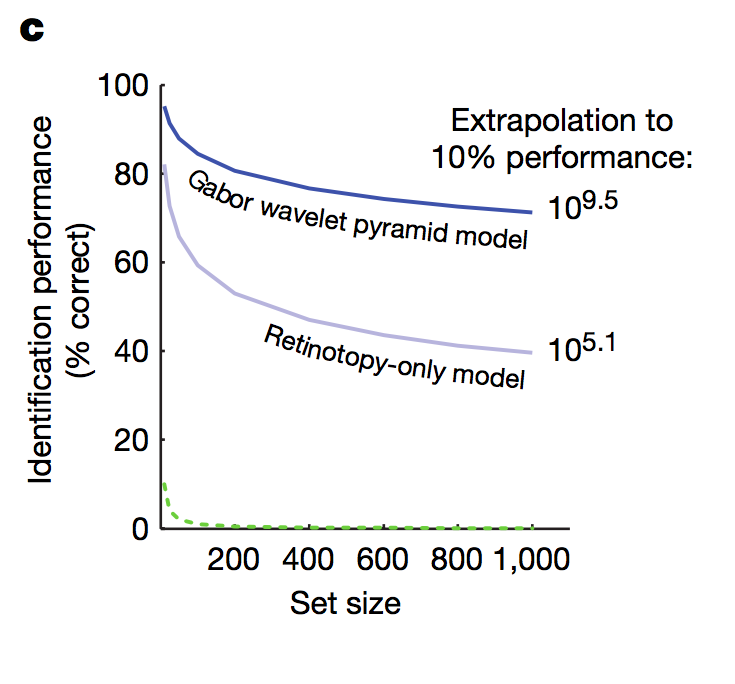
\includegraphics[scale = 0.2, clip=true, trim = 0 0in 0 0]{kay_extrapolation.png}
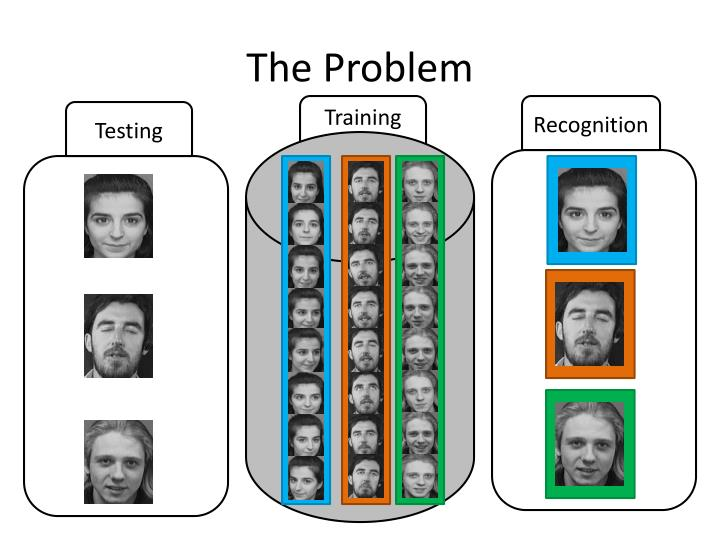
\includegraphics[scale = 0.2]{face_rec_the-problem-n.jpg}\pause
\hspace{0.2in}
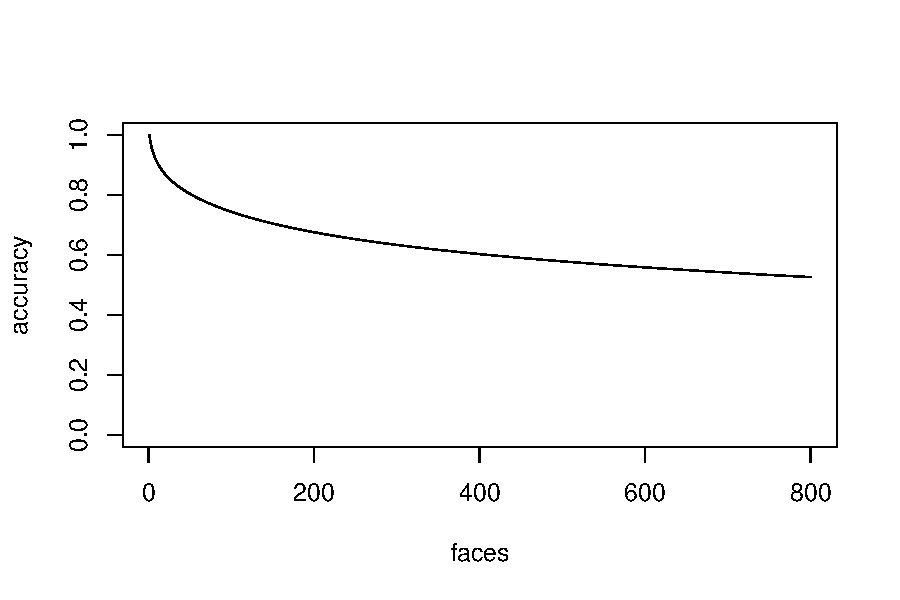
\includegraphics[scale = 0.3]{../facerec/acc_plot1.pdf}\pause
\end{center}

How does the accuracy scale with the number of classes (faces)?
\end{frame}




\begin{frame}
\frametitle{Setup}

\begin{center}
\begin{tabular}{c|c}
1. Population of categories $\pi(y)$ & 
2. Subsample $k$ labels, $y_1,\hdots, y_k$\\
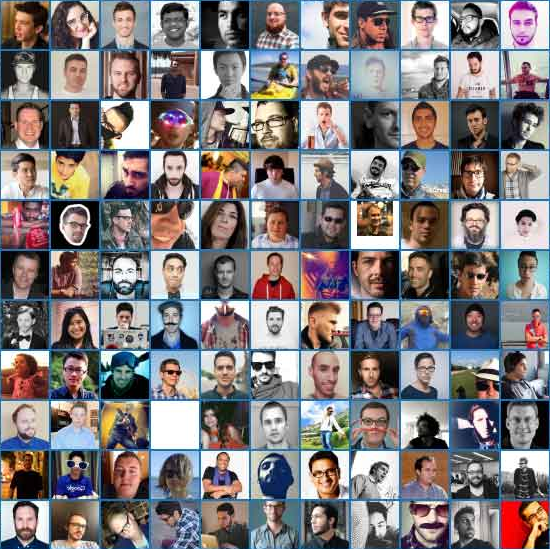
\includegraphics[scale = 0.2]{facegrid.png} &
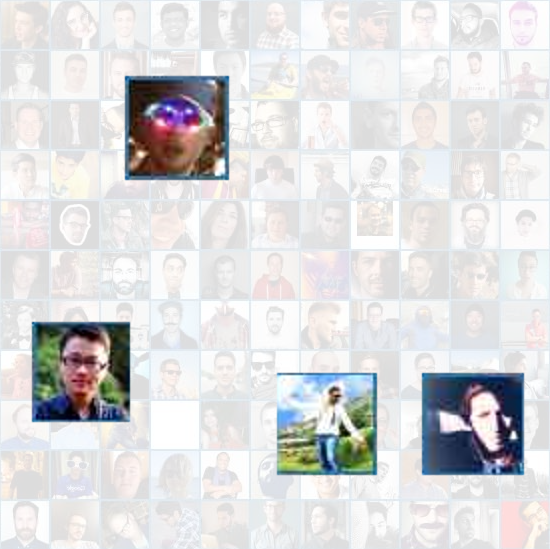
\includegraphics[scale = 0.2]{facegrid_samp.png}
\end{tabular}
\end{center}

\pause

\vspace{0.1in}
3. Collect training and test data $x_i^{(j)}$ (faces) for labels (people) $\{y_1,\hdots, y_k\}$.\pause

\vspace{0.1in}
4. Train a classifier and compute test error. \pause

\vspace{0.1in}
\textbf{Can we analyze how error depends on }$k$?
\end{frame}


\begin{frame}
\frametitle{Key assumption: marginal classifier}
\begin{itemize}
\item The classifier is \emph{marginal} if it learns a model \emph{independently} for each class.\pause
\item Examples: LDA/QDA 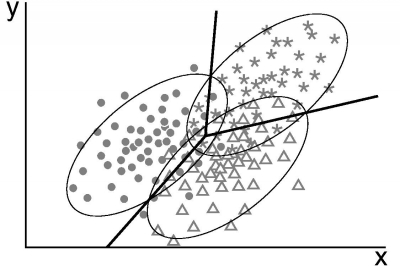
\includegraphics[scale = 0.2]{discriminant.jpg}, \pause
na\"{i}ve Bayes 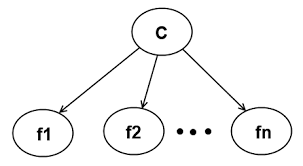
\includegraphics[scale = 0.2]{naive_bayes.png}
\item Non-marginal classifiers: Multinomial logistic, multilayer neural networks, k-nearest neighbors
\end{itemize}
\end{frame}

\begin{frame}
\frametitle{Definitions}

$\hat{F}_{y^{(i)}}$ is the empirical distribution obtained from the training data for label $y^{(i)}$.

\begin{center}
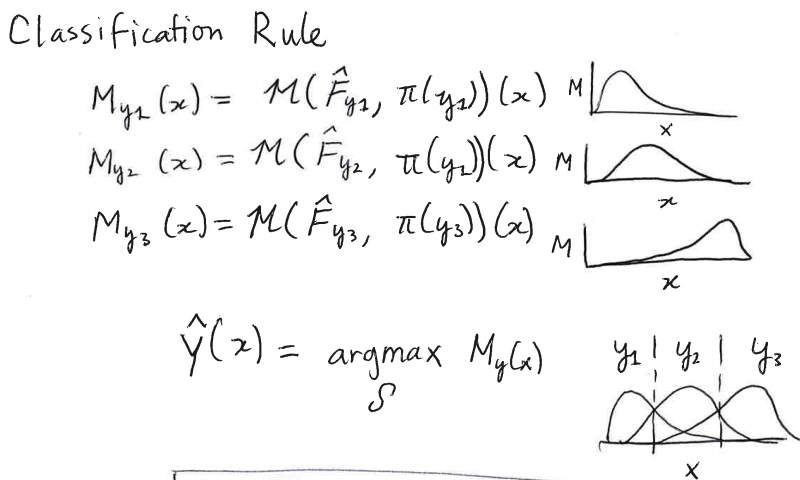
\includegraphics[scale = 0.2]{../info_theory_paper/extrapolation_figures/classification_rule.png}
\end{center}
\end{frame}

\begin{frame}

\begin{center}
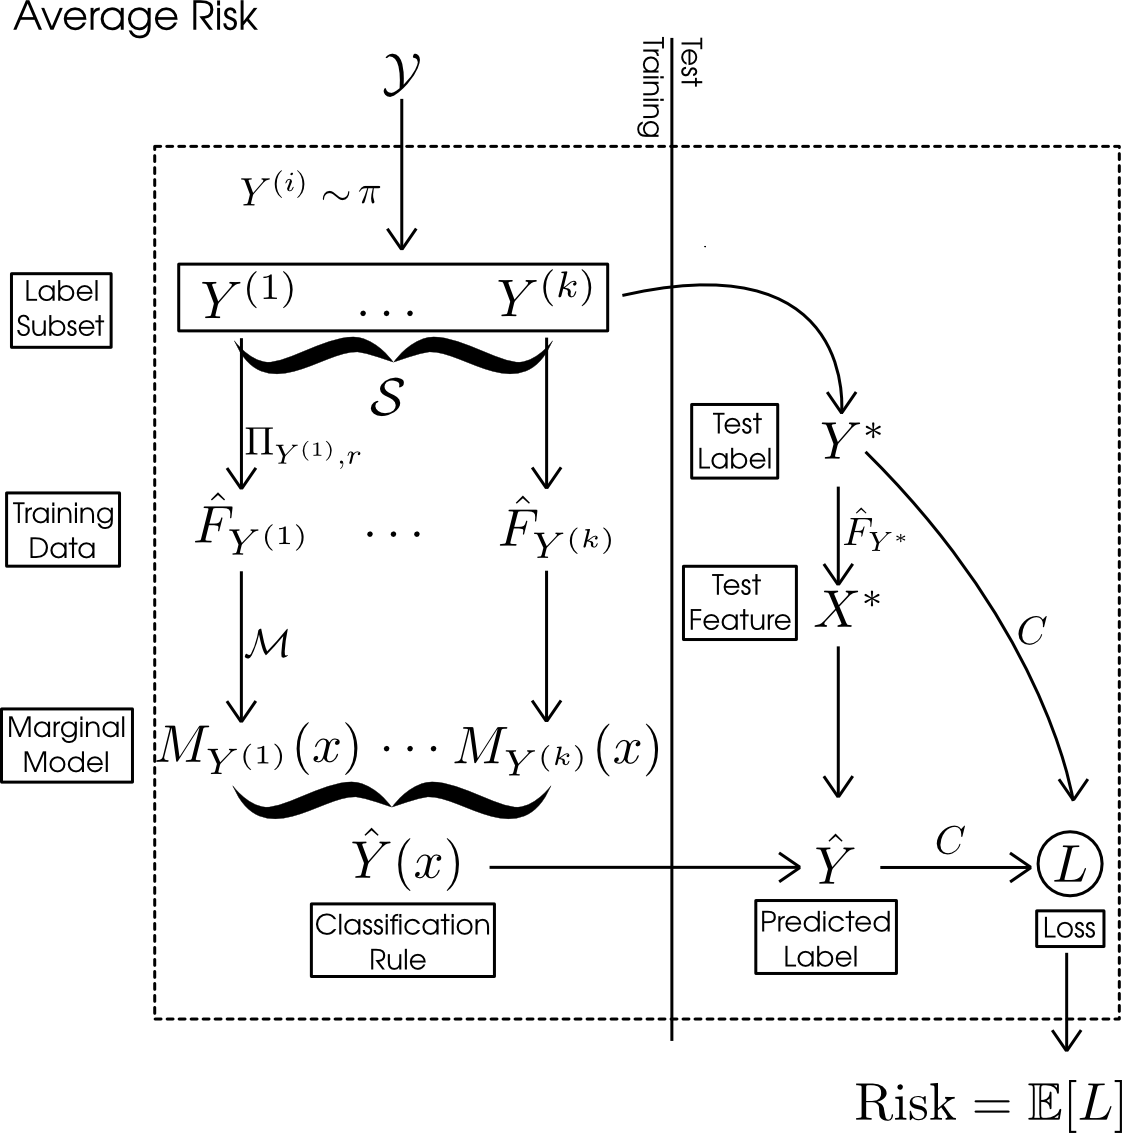
\includegraphics[scale = 0.2]{../info_theory_paper/extrapolation_figures/average_risk.png}
\end{center}
\end{frame}


\begin{frame}
\frametitle{Theoretical Result}

\textbf{Theorem. (Z.}, Achanta, Benjamini.)
Suppose $\pi$, $\{F_y\}_{y \in \mathcal{Y}}$ and marginal classifier
$\mathcal{F}$ satisfy \emph{(some regularity condition)}.  Then, 
there exists some function $\bar{D}(u)$ on $[0,1] \to [0,1]$ such that
the $k$-class average risk is given by
\begin{equation}\label{eq:avrisk_identity}
\text{AvRisk}_k = (k-1) \int \bar{D}(u) u^{k-2} du.
\end{equation}
\pause

\vspace{1in}
What is this $\bar{D}(u)$ function? We will explain in the following toy example...
\end{frame}

\begin{frame}
\frametitle{Toy example}
$Y_1,\hdots, Y_k \stackrel{iid}{\sim} N(0, 1);$\pause

$X|Y \sim N(\rho Y, 1-\rho^2)$ i.e. $(Y, X) \sim N(0, \begin{pmatrix}1 & \rho\\\rho & 1\end{pmatrix}).$

\begin{center}
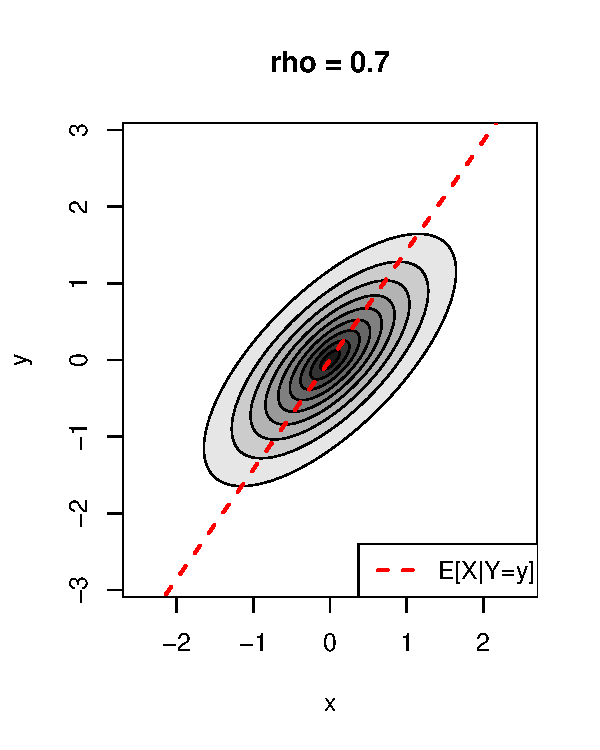
\includegraphics[scale = 0.5, clip = true, trim = 0 0 0 0.5in]{../extrapolation/illus_rho_0_7.pdf}
\end{center}

\end{frame}





\begin{frame}
\frametitle{Toy example}

\begin{center}
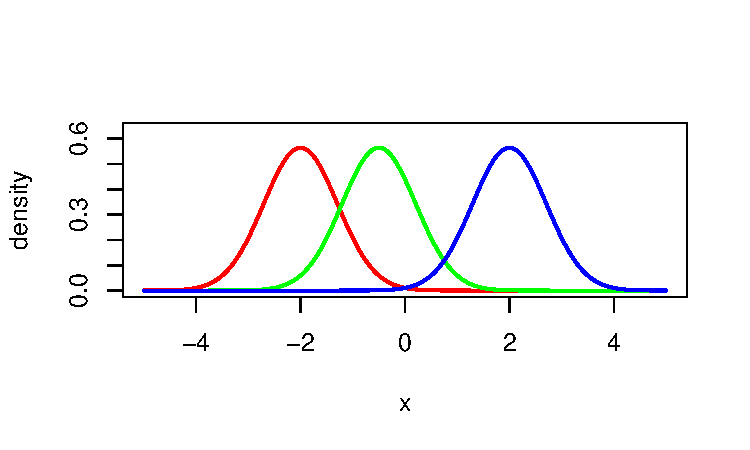
\includegraphics[scale = 0.5, clip = true, trim = 0 0.8in 0 0.8in]{../extrapolation/illus_example1a.pdf}
\end{center}

\begin{itemize}
\item Suppose $k=3$, and we draw $Y_1, Y_2, Y_3$.
\item The \emph{Bayes rule} is the optimal classifier and depends on knowing the true densities:
\[
\hat{y}(x) = \text{argmax}_{y_i} p(x|y_i)
\]
\item The \emph{Bayes Risk}, which is the misclassification rate of the optimal classifier.
\end{itemize}

\end{frame}

\begin{frame}
\frametitle{Toy example}

\begin{center}
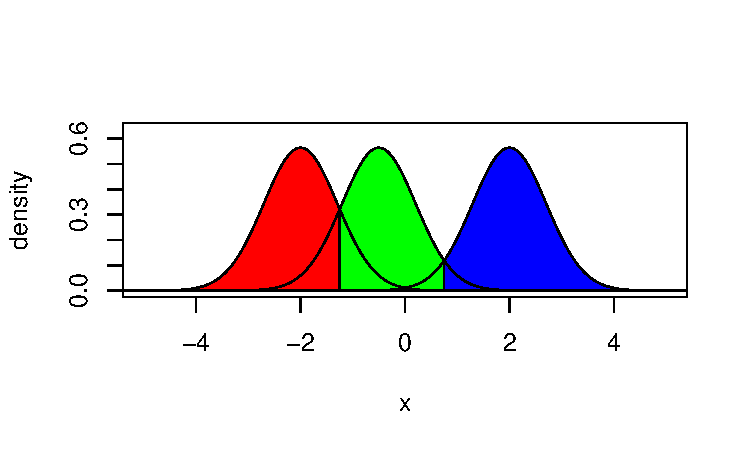
\includegraphics[scale = 0.5, clip = true, trim = 0 0 0 0.5in]{../extrapolation/illus_example1b.pdf}
\end{center}

\begin{itemize}
\item The \emph{Bayes Risk} is the expected test error of the Bayes rule,
\[
\frac{1}{k} \sum_{i=1}^k \Pr[\hat{y}(x) \neq Y| Y = y_i]
\]
\end{itemize}
% = 1 - \frac{1}{k}\int \max_{i=1}^k p(x|y_i) dx.

\end{frame}

\begin{frame}
\frametitle{Toy example}
\begin{columns}
\begin{column}{0.5\textwidth}
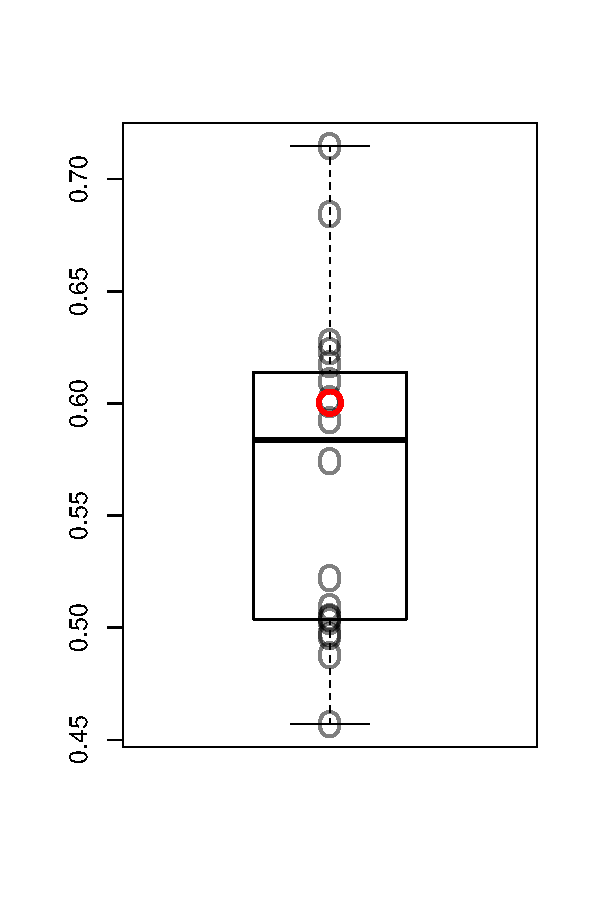
\includegraphics[scale = 0.5]{../extrapolation/autoplots/box4_1.pdf}
\end{column}
\begin{column}{0.5\textwidth}
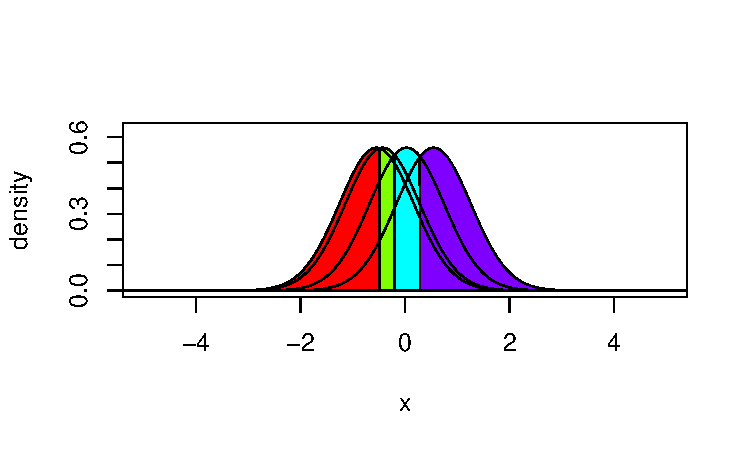
\includegraphics[scale = 0.5]{../extrapolation/autoplots/dens4_1.pdf}
\end{column}
\end{columns}
\end{frame}

\begin{frame}
\frametitle{Toy example}
\begin{columns}
\begin{column}{0.5\textwidth}
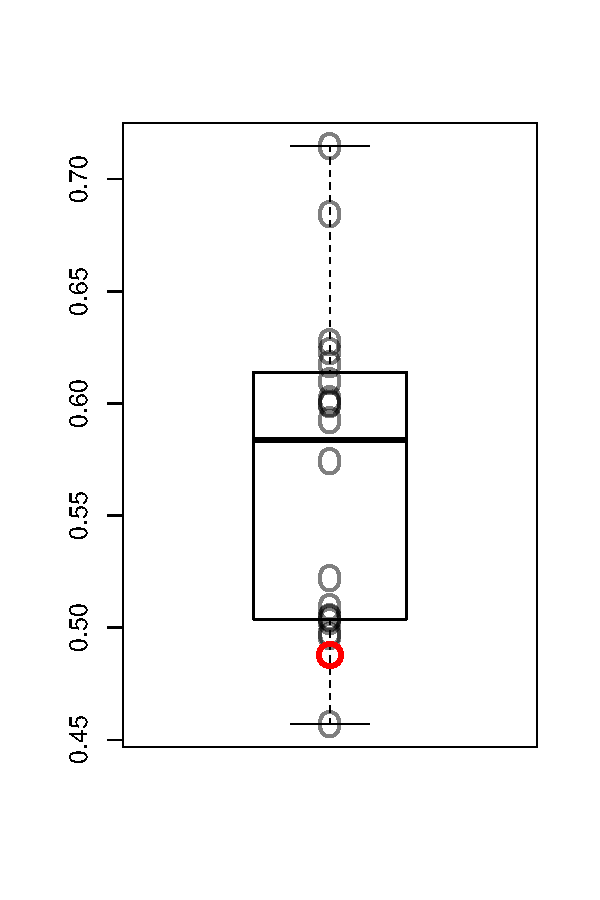
\includegraphics[scale = 0.5]{../extrapolation/autoplots/box4_2.pdf}
\end{column}
\begin{column}{0.5\textwidth}
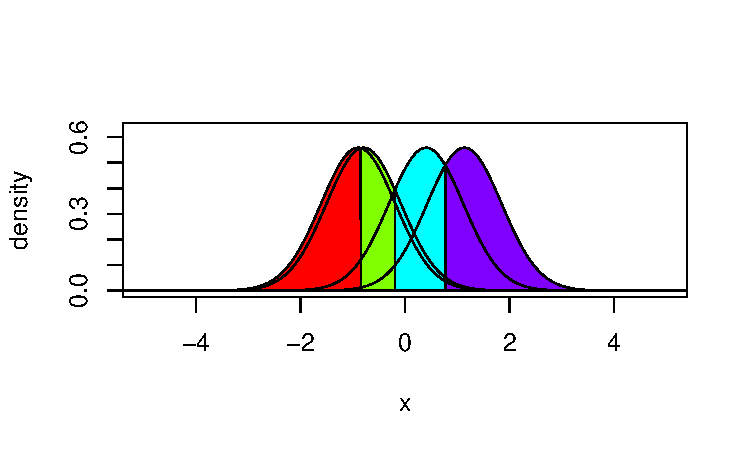
\includegraphics[scale = 0.5]{../extrapolation/autoplots/dens4_2.pdf}
\end{column}
\end{columns}
\end{frame}

\begin{frame}
\frametitle{Toy example}
\begin{columns}
\begin{column}{0.5\textwidth}
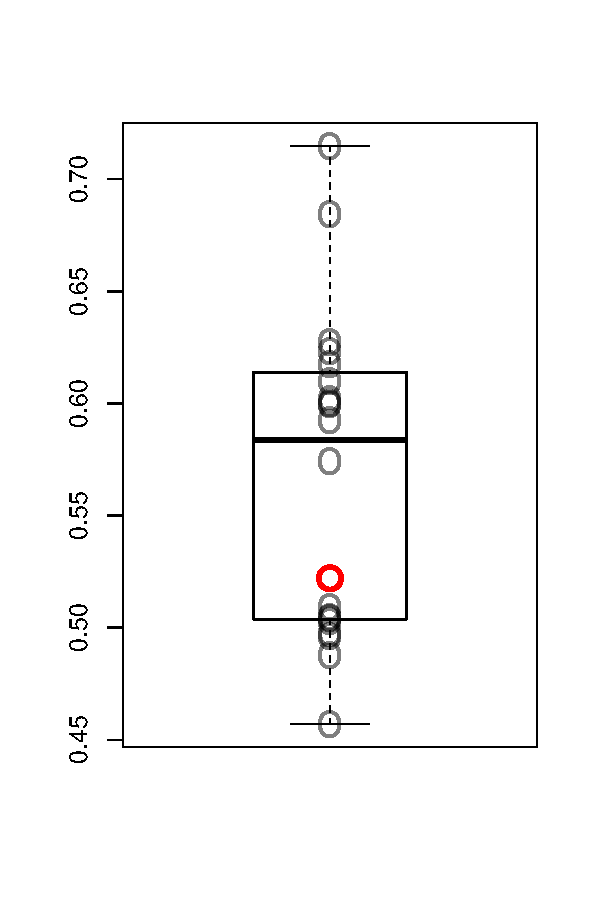
\includegraphics[scale = 0.5]{../extrapolation/autoplots/box4_3.pdf}
\end{column}
\begin{column}{0.5\textwidth}
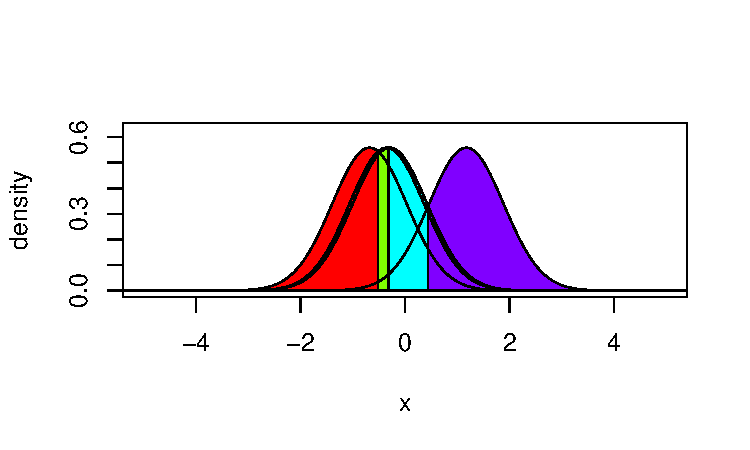
\includegraphics[scale = 0.5]{../extrapolation/autoplots/dens4_3.pdf}
\end{column}
\end{columns}
\end{frame}

\begin{frame}
\frametitle{Toy example}
\begin{center}
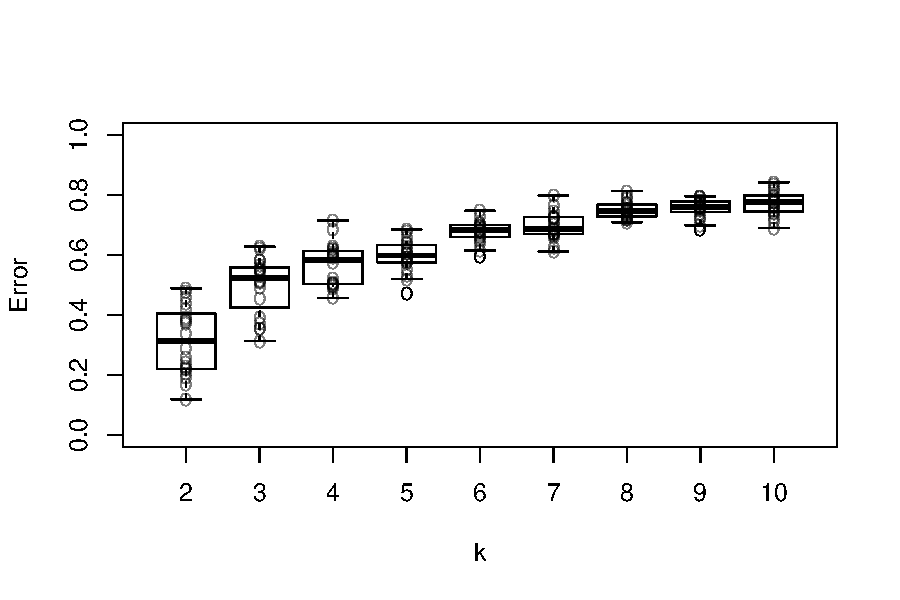
\includegraphics[scale = 0.5]{../extrapolation/autoplots/all_box.pdf}
\end{center}
\end{frame}

\begin{frame}
\frametitle{Toy example}
\begin{center}
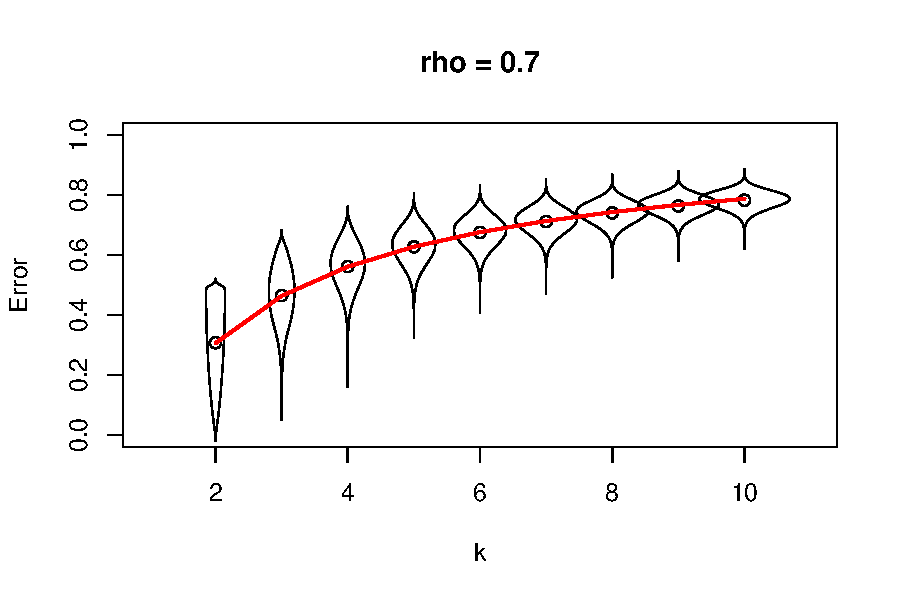
\includegraphics[scale = 0.5]{../extrapolation/illus_err_0_7.pdf}
\end{center}
\end{frame}

\begin{frame}
\frametitle{Defining the $U$-function}
Define $U_x(y)$ as follows:
\begin{itemize}
\item Suppose we have test instance (face) $x$ whose true label (person) is $y$.
\item Let $Y'$ be a random \emph{incorrect} label (person).
\item Use the classifier to guess whether $x$ belongs to $y$ or $Y'$.
\item Define $U_x(y)$ as the probabilility of success (randomizing over training data).
\end{itemize}
\end{frame}

\begin{frame}
\frametitle{Toy example}
\begin{center}
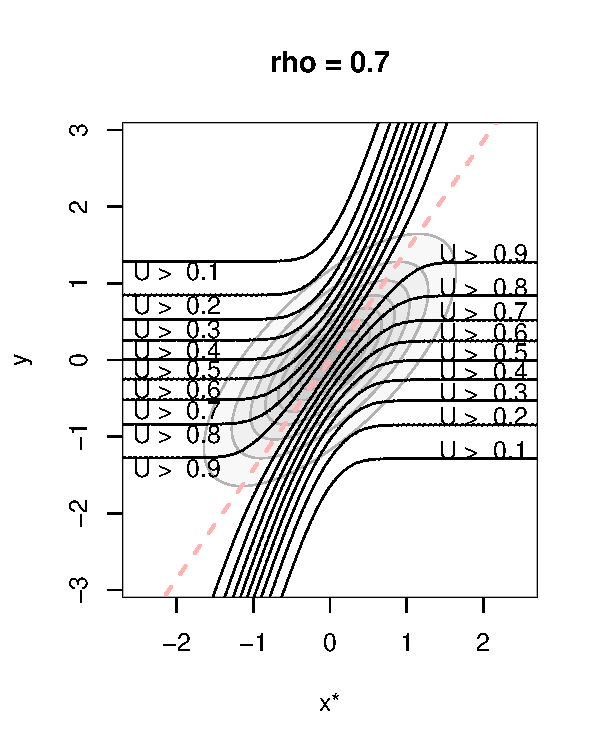
\includegraphics[scale = 0.5]{../extrapolation/illus_ufunc_0_7.pdf}
\end{center}
\[
U_y(x) = \Pr[d(x, \rho Y') > d(x, \rho y)],\text{ for }Y' \sim N(0,1).
\]
\end{frame}

\begin{frame}
\frametitle{Defining the $\bar{D}(u)$}
\begin{itemize}
\item Define random variable as $U_Y(X)$ for $(Y, X)$ drawn from the joint distribution.\pause
\item $\bar{D}(u)$ is the cumulative distribution function of $U$,
\[
\bar{D}(u) = \Pr[U_Y(X) \leq u].
\]
\pause
\end{itemize}
\begin{center}
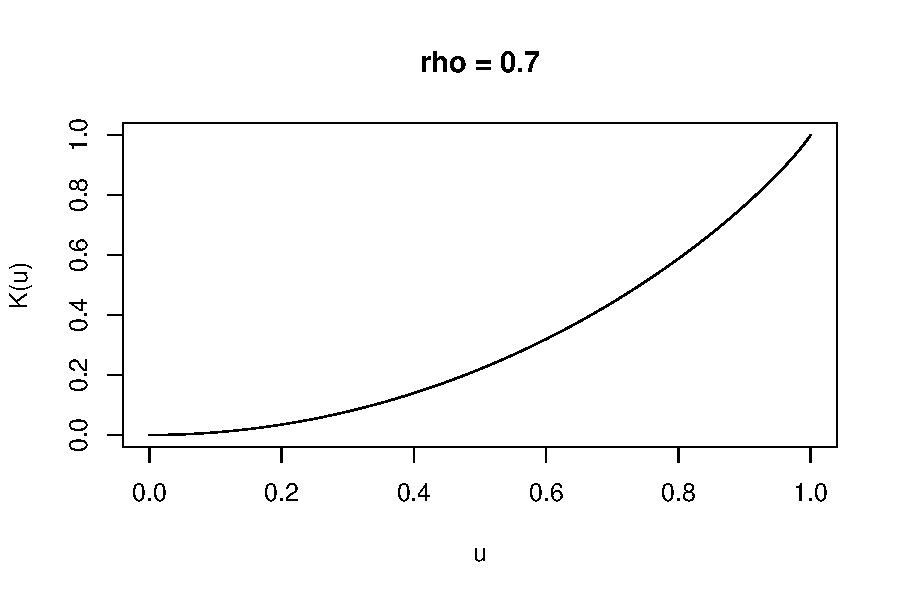
\includegraphics[scale = 0.45]{../extrapolation/illus_kfunc_0_7.pdf}
\end{center}
\end{frame}



\end{document}
\end{frame}
\end{document}






















\begin{frame}
\frametitle{Considering the $k=2$ case}
How is the risk in $k=2$ case defined?
\begin{itemize}
\item[1.] Draw $Y_1, Y_2 \sim N(0, 1)$.
\item[2.] Flip a coin to choose a class $i \in \{1,2\}$.
\item[3.] Draw $X$ from the $i$th class, $X \sim p(x|y_i)$.
\end{itemize}
\end{frame}

\begin{frame}
\frametitle{Considering the $k=2$ case}
How is the risk in $k=2$ case defined?
\begin{itemize}
\item[1.] Draw $Y_1, Y_2 \sim N(0, 1)$.
\item[2.] \textcolor{red}{WLOG} assume the true class is $i = 1$. 
\item[3.] Draw $X$ from the \textcolor{red}{first} class, $X \sim p(x|y_{\textcolor{red}{1}})$. \pause
\item[4.] Correct classification if $p(X|y_1) > p(X|y_2)$.
\end{itemize}
\end{frame}

\begin{frame}
\frametitle{Considering the $k=2$ case}
How is the risk in $k=2$ case defined?
\begin{itemize}
\item[1.] Draw $Y_1, Y_2 \sim N(0, 1)$.
\item[2.] WLOG assume the true class is $i = 1$. 
\item[3.] Draw $X$ from the first class, $X \sim p(x|y_1)$. \pause
\item[4.] Correct classification if $|X - \rho y_1| < |X - \rho y_2|$.\pause
\end{itemize}

The Bayes risk for labels $y_1, y_2$ is
\[
\text{Risk}(y_1, y_2) = \Pr[|X - \rho y_1| < |X - \rho y_2|].
\]
\end{frame}

\begin{frame}
\frametitle{Considering the $k=2$ case}
How is the risk in $k=2$ case defined?
\begin{itemize}
\item[1.] Draw $Y_1, Y_2 \sim N(0, 1)$.
\item[2.] WLOG assume the true class is $i = 1$. 
\item[3.] Draw $X$ from the first class, $X \sim p(x|y_1)$.
\item[4.] Correct classification if $|X - \rho y_1| < |X - \rho y_2|$.
\end{itemize}

The \textcolor{red}{\emph{average}} Bayes Risk for $k = 2$ is
\[
\text{AvRisk}_2 = \E[\text{Risk}(Y_1, Y_2)] = \Pr[|X - \rho Y_1| < |X - \rho Y_2|].
\]
for $X \sim N(\rho Y_1, 1-\rho^2)$.
\end{frame}

\begin{frame}
\frametitle{Considering the $k=2$ case}
The main theoretical trick we use is to change the order of conditioning.

\end{frame}
